\documentclass[11pt,a4paper]{report}

%------------------------------------------------------------------
% Packages
%------------------------------------------------------------------
\usepackage[a4paper, top=0.9in, bottom=0.9in, left=1.1in, right=0.9in]{geometry}
\usepackage{amsmath, amssymb}
\usepackage{graphicx}
\usepackage{booktabs}
\usepackage{array}
\usepackage{longtable}
\usepackage{hyperref}
\usepackage{setspace}
\usepackage{fancyhdr}
\usepackage{titlesec}
\usepackage{caption}
\usepackage{subcaption}
\usepackage{enumitem}
\usepackage{xcolor}
\usepackage{tikz}
\usepackage{pgfplots}
\pgfplotsset{compat=1.18}
\usetikzlibrary{arrows.meta, positioning, shapes.geometric, fit, backgrounds}
\usepackage{float}
\usepackage{multirow}

\hypersetup{
    colorlinks=true,
    linkcolor=blue!60!black,
    citecolor=green!50!black,
    urlcolor=blue!60!black,
    pdftitle={Room Digital Twin: A Real-Time 3D Thermal Simulation Framework},
    pdfauthor={Mobashshir Zainuddin},
    bookmarks=true,
    bookmarksopen=true,
    pdfpagemode=UseOutlines
}

\singlespacing

\pagestyle{fancy}
\fancyhf{}
\fancyhead[L]{\small\nouppercase{\leftmark}}
\fancyhead[R]{\small Room Digital Twin}
\fancyfoot[C]{\thepage}
\renewcommand{\headrulewidth}{0.4pt}

\titleformat{\chapter}[hang]
  {\normalfont\large\bfseries}
  {\thechapter}{1em}{}
\titlespacing*{\chapter}{0pt}{6pt}{8pt}

\titleformat{\section}
  {\normalfont\normalsize\bfseries}{\thesection}{1em}{}
\titlespacing*{\section}{0pt}{6pt}{3pt}

\titleformat{\subsection}
  {\normalfont\small\bfseries}{\thesubsection}{1em}{}
\titlespacing*{\subsection}{0pt}{4pt}{2pt}

\usepackage{etoolbox}
\makeatletter
\patchcmd{\chapter}{\if@openright\cleardoublepage\else\clearpage\fi}{}{}{}
\makeatother

\setlist{noitemsep, topsep=2pt, partopsep=0pt}

\captionsetup{font=small, skip=4pt}

\makeatletter
\renewcommand\listoffigures{%
  \section*{\listfigurename}%
  \@mkboth{\MakeUppercase\listfigurename}{\MakeUppercase\listfigurename}%
  \@starttoc{lof}%
}
\renewcommand\listoftables{%
  \section*{\listtablename}%
  \@mkboth{\MakeUppercase\listtablename}{\MakeUppercase\listtablename}%
  \@starttoc{lot}%
}
\makeatother

%==================================================================
\begin{document}
%==================================================================

%------------------------------------------------------------------
% Title Page
%------------------------------------------------------------------
\begin{titlepage}
\centering
\vspace*{1cm}

{\large\bfseries INDIAN INSTITUTE OF TECHNOLOGY KHARAGPUR}

\vspace{0.8cm}

\includegraphics[width=5cm]{iitkharagpur_logo.png}

\vspace{0.8cm}
{\LARGE\bfseries Room Digital Twin: A Real-Time 3D Thermal\\ and Psychrometric Simulation Framework}

\vspace{0.8cm}
{\large Report submitted to}\\[0.3cm]
{\Large\bfseries Indian Institute of Technology Kharagpur}

\vspace{0.6cm}
{\normalsize In partial fulfilment of the requirements for the award of the degree of}\\[0.3cm]
{\large\bfseries B.Tech.\ in Mining Engineering and M.Tech.\ in Petroleum Engineering}

\vspace{0.8cm}
{\normalsize By}\\[0.3cm]
{\Large\bfseries Mobashshir Zainuddin}\\[0.2cm]
{\Large\bfseries 23MI3PE01}

\vspace{0.6cm}
{\normalsize Under the guidance of}\\[0.4cm]
{\Large\bfseries Prof.\ Mohammad Saud Afzal}\\
\vspace{0.3cm}
{\large\bfseries Civil Engineering Department}\\
\vspace{0.4cm}
{\large\bfseries November 2026}

\vspace{0.3cm}
{\small \copyright\ 2026, Mobashshir Zainuddin. All rights reserved.}

\end{titlepage}

%------------------------------------------------------------------
% Declaration
%------------------------------------------------------------------
\thispagestyle{plain}
\chapter*{\underline{DECLARATION}}
\addcontentsline{toc}{chapter}{Declaration}

I certify that
\begin{enumerate}[label=\alph*.]
  \item the work contained in this report is original and has been done by me under the guidance of my supervisor(s).
  \item the work has not been submitted to any other Institute for any degree or diploma.
  \item I have followed the guidelines provided by the Institute in preparing the report.
  \item I have conformed to the norms and guidelines given in the Ethical Code of Conduct of the Institute.
  \item Whenever I have used materials from other sources, I have given due credit by citing them in the text and listing them in the references.
\end{enumerate}

\vspace{2cm}
\hfill Signature of the Student

\newpage

%------------------------------------------------------------------
% Certificate
%------------------------------------------------------------------
\thispagestyle{plain}
\chapter*{\underline{CERTIFICATE}}
\addcontentsline{toc}{chapter}{Certificate}

\vspace{0.5cm}
\noindent This is to certify that the Report entitled, ``\textbf{Room Digital Twin: A Real-Time 3D Thermal and Psychrometric Simulation Framework}'' submitted by \textbf{Mr.\ Mobashshir Zainuddin} to IIT Kharagpur is a record of bonafide Project work carried out under my supervision and is worthy of consideration for the award of B.Tech.\ in Mining Engineering and M.Tech.\ in Petroleum Engineering.

\vspace{3cm}
\noindent\rule{6cm}{0.4pt}\\
Prof.\ Mohammad Saud Afzal\\
Civil Engineering Department\\
Supervisor

\vspace{0.8cm}
\noindent Date: November 2026

\newpage

%------------------------------------------------------------------
% Acknowledgements
%------------------------------------------------------------------
\thispagestyle{plain}
\chapter*{Acknowledgements}
\addcontentsline{toc}{chapter}{Acknowledgements}

I am deeply grateful to \textbf{Prof.\ Mohammad Saud Afzal}, Civil Engineering Department, IIT Kharagpur, for his continuous guidance and encouragement. I also thank \textbf{Mr.\ Ali Shariq} for his valuable assistance on numerical methods and psychrometric calculations. Finally, I express sincere gratitude to my family and friends for their constant moral support.

\vspace{1.5cm}
\begin{flushright}
Mobashshir Zainuddin\\
23MI3PE01\\
Mining Engineering Department\\
November 2026
\end{flushright}

\newpage

%------------------------------------------------------------------
% Abstract
%------------------------------------------------------------------
\chapter*{Abstract}
\addcontentsline{toc}{chapter}{Abstract}

This report presents the \textbf{Room Digital Twin}, a browser-based application that simulates the coupled thermodynamic and psychrometric behaviour of a conditioned room in real time. Its core is a 3D Finite Difference Method (FDM) engine on a Cartesian grid with explicit Forward Euler time-stepping governed by the CFL criterion, which transports heat, moisture ratio, and three velocity components. A complete psychrometric engine computes saturation vapour pressure, humidity ratio, relative humidity, dew point, wet-bulb temperature (Stull 2011), specific enthalpy (ASHRAE), and moist-air density for every cell at every step. Buoyancy-driven convection is captured through the Boussinesq approximation. The application is packaged as an Electron.js desktop app with a Three.js 3D scene, a probe tool, and a heat-map visualisation. Future work proposes replacing the FDM solver with Physics-Informed Neural Networks (PINNs).

\vspace{0.5cm}
\noindent\textbf{Keywords:} Digital Twin, FDM, Psychrometrics, Building Energy Simulation, Boussinesq, HVAC, Three.js, Electron.js.

\newpage

%------------------------------------------------------------------
% Table of Contents
%------------------------------------------------------------------
\tableofcontents
\listoffigures
\addcontentsline{toc}{chapter}{List of Figures}
\vspace{1em}
\listoftables
\addcontentsline{toc}{chapter}{List of Tables}
\newpage

%==================================================================
\chapter{Introduction}
\label{ch:intro}
%==================================================================

Buildings account for $\approx$36\% of global final energy consumption \cite{iea2022}; space conditioning dominates, often 50--70\% of a building's energy bill \cite{ashrae2021}. Traditional tools such as EnergyPlus \cite{crawley2001} and CFD solvers are accurate but require hours of offline computation, making them unsuitable for real-time operational decisions. A \textbf{digital twin}, a virtual replica synchronised with its physical counterpart \cite{grieves2014}, offers an alternative in which a lightweight physics engine coupled with a live 3D scene allows building operators to explore what-if scenarios in real time.

\section{Related Work}
\label{sec:lit}

EnergyPlus \cite{crawley2001} and DOE-2 \cite{winkelmann1993} are the standard whole-building energy simulation tools; their turnaround of minutes-to-hours precludes real-time use. Reduced-order models (POD \cite{pod2002}, DMD) pre-compute a compact basis for fast online evaluation but require expensive offline training. Commercial digital twin platforms (Siemens MindSphere, IBM Maximo) handle synchronisation and analytics but delegate physics to third-party solvers. Academic prototypes such as Zhao et al.\ \cite{zhao2020} and Deng et al.\ \cite{deng2022} couple physics-informed data-driven models with IoT sensor networks. The present work uses a fully client-side FDM solver in JavaScript running on a standard laptop with no offline pre-computation.

\section{Objectives}
\label{sec:objectives}

\begin{enumerate}
  \item Develop a 3D FDM physics engine solving coupled heat, moisture, and momentum transport on a Cartesian grid in real time.
  \item Implement a complete ASHRAE psychrometric engine: saturation pressure, humidity ratio, RH, dew point, wet-bulb, enthalpy, and moist-air density.
  \item Model physically realistic boundary conditions: wall conduction, solar gain, AC supply, occupant and equipment loads, infiltration, and door-driven exchange.
  \item Render the room in a Three.js 3D scene with a probe tool and temperature heat-map mode.
  \item Package the application as a standalone Electron.js desktop app.
\end{enumerate}





%==================================================================
\chapter{Theoretical Background}
\label{ch:theory}
%==================================================================

\section{Governing Transport Equations}
\label{sec:govern}

Indoor air is treated as an incompressible Newtonian fluid under the low-Mach-number approximation. Three scalar fields are transported: temperature $T$ [°C], humidity ratio $\omega$ [kg$_w$/kg$_{da}$], and velocity $(u,v,w)$ [m/s].

\subsection{Heat Transport}

\begin{equation}
  \frac{\partial T}{\partial t} = \alpha\,\nabla^2 T - \mathbf{v}\cdot\nabla T + S_T
  \label{eq:heat}
\end{equation}

where $\alpha \approx 22\times10^{-6}$\,m$^2$/s is the thermal diffusivity of air and $S_T$ [°C/s] aggregates wall conduction, solar gain, occupant metabolic heat, equipment loads, and AC injection.

\subsection{Moisture Transport}

\begin{equation}
  \frac{\partial \omega}{\partial t} = D_m\,\nabla^2\omega - \mathbf{v}\cdot\nabla\omega + S_\omega
  \label{eq:moisture}
\end{equation}

where $D_m \approx 25\times10^{-6}$\,m$^2$/s and $S_\omega$ includes infiltration, occupant transpiration, and AC dehumidification.

\subsection{Momentum and Boussinesq Approximation}

\begin{equation}
  \frac{\partial \mathbf{v}}{\partial t} = \nu\,\nabla^2\mathbf{v} - (\mathbf{v}\cdot\nabla)\mathbf{v} + \mathbf{g}\,\beta\,(T - T_\text{ref})
  \label{eq:momentum}
\end{equation}

where $\nu \approx 15\times10^{-6}$\,m$^2$/s, $\beta = 1/(T_\text{ref}+273.15)$\,K$^{-1}$, and $\mathbf{g}=(0,-g,0)$. The Boussinesq approximation \cite{boussinesq1903} neglects density differences everywhere except the buoyancy term, which is valid for $\Delta T/T_\text{ref}\ll1$. After each velocity update a damping factor $d=0.97$ is applied:

\begin{equation}
  \mathbf{v}^{n+1} \leftarrow d\,\mathbf{v}^{n+1}
  \label{eq:damping}
\end{equation}

Velocity components are additionally capped at $\pm0.8$\,m/s (horizontal) and $\pm0.6$\,m/s (vertical).

\section{Psychrometric Relations}
\label{sec:psychro}

\subsection{Saturation Vapour Pressure (Magnus Formula)}

\begin{equation}
  \boxed{p_{ws}(T) = 610.78\exp\!\left(\frac{17.27\,T}{T + 237.3}\right)}
  \label{eq:magnus}
\end{equation}

The formula is accurate to within 0.3\% over $-30$°C to $+60$°C \cite{august1828,alduchov1996}.

\subsection{Partial Pressure and Humidity Ratio}

\begin{equation}
  \omega = 0.621945\,\frac{p_v}{P - p_v} \quad\Longrightarrow\quad p_v = \frac{\omega\,P}{\omega + 0.621945}
  \label{eq:omega}
\end{equation}

where $P = 101325$\,Pa \cite{ashrae2021}.

\subsection{Relative Humidity}

\begin{equation}
  \phi = \frac{p_v}{p_{ws}(T)} \times 100\%
  \label{eq:rh}
\end{equation}

\subsection{Dew-Point Temperature}

\begin{equation}
  \boxed{T_{dp} = \frac{237.3\,\ln(p_v/610.78)}{17.27 - \ln(p_v/610.78)}}
  \label{eq:tdp}
\end{equation}

\subsection{Wet-Bulb Temperature (Stull 2011)}

\begin{equation}
\begin{aligned}
  T_{wb} &= T\arctan\!\left(0.151977\sqrt{\phi + 8.313659}\right) + \arctan(T + \phi)\\
  &\quad - \arctan(\phi - 1.676331) + 0.00391838\,\phi^{3/2}\arctan(0.023101\,\phi) - 4.686035
\end{aligned}
  \label{eq:twb}
\end{equation}

Accurate to $\pm0.65$°C for $0\leq T\leq40$°C and $5\leq\phi\leq99\%$ \cite{stull2011}.

\subsection{Specific Enthalpy}

\begin{equation}
  \boxed{h = 1.006\,T + \omega\,(2501 + 1.86\,T)}
  \label{eq:enthalpy}
\end{equation}

\cite{ashrae2021}.

\subsection{Moist-Air Density}

\begin{equation}
  \boxed{\rho = \frac{P - p_v}{R_{da}\,T_K} + \frac{p_v}{R_v\,T_K}}
  \label{eq:density}
\end{equation}

where $T_K = T+273.15$\,K, $R_{da}=287.058$\,J/(kg·K), $R_v=461.495$\,J/(kg·K).

\section{Numerical Methods}
\label{sec:numerics}

\subsection{FDM Discretisation}

The domain $[0,L_x]\times[0,L_y]\times[0,L_z]$ is divided into $N_x\times N_y\times N_z$ uniform cells. The Laplacian uses the standard second-order central-difference stencil:

\begin{equation}
  (\nabla^2 f)_{i,j,k} \approx \frac{f_{i+1,j,k} - 2f_{i,j,k} + f_{i-1,j,k}}{\Delta x^2}
  + \frac{f_{i,j+1,k} - 2f_{i,j,k} + f_{i,j-1,k}}{\Delta y^2}
  + \frac{f_{i,j,k+1} - 2f_{i,j,k} + f_{i,j,k-1}}{\Delta z^2}
  \label{eq:laplacian}
\end{equation}

Advection uses the first-order upwind scheme:

\begin{equation}
  (u\,\partial_x f)_{i,j,k} \approx
  u^+\,\frac{f_{i,j,k} - f_{i-1,j,k}}{\Delta x} + u^-\,\frac{f_{i+1,j,k} - f_{i,j,k}}{\Delta x}
  \label{eq:upwind}
\end{equation}

where $u^+=\max(u,0)$ and $u^-=\min(u,0)$.

\subsection{Forward Euler Time Integration}

\begin{equation}
  f^{n+1}_{i,j,k} = f^n_{i,j,k} + \Delta t\,\mathcal{L}(f^n)_{i,j,k}
  \label{eq:euler}
\end{equation}

Double buffering (two \texttt{Float32Array} arrays) prevents read-write conflicts.

\subsection{CFL Stability Criterion}

\begin{equation}
  \Delta t \leq \min\!\left(\frac{\Delta x^2}{2\alpha}, \frac{\Delta y^2}{2\alpha}, \frac{\Delta z^2}{2\alpha},
  \frac{\Delta x}{|u|_\text{max}}, \frac{\Delta y}{|v|_\text{max}}, \frac{\Delta z}{|w|_\text{max}}\right)
  \label{eq:cfl}
\end{equation}

The solver enforces $\Delta t_\text{max}=0.15$\,s empirically \cite{courant1928}. Up to 32 physics sub-steps execute per animation frame.





%==================================================================
\chapter{Methodology and Implementation}
\label{ch:impl}
%==================================================================

\section{System Architecture}
\label{sec:arch}

The application comprises four coupled layers (Figure~\ref{fig:arch}), namely a UI layer (parameter panel, probe, 3D canvas), a Three.js rendering layer, an FDM physics engine on a Cartesian grid using \texttt{Float32Array}, and a psychrometric engine. Electron.js \cite{electron} embeds the Chromium renderer and Node.js runtime in a desktop executable. The same HTML/JavaScript source runs in a browser during development.

\begin{figure}[H]
\centering
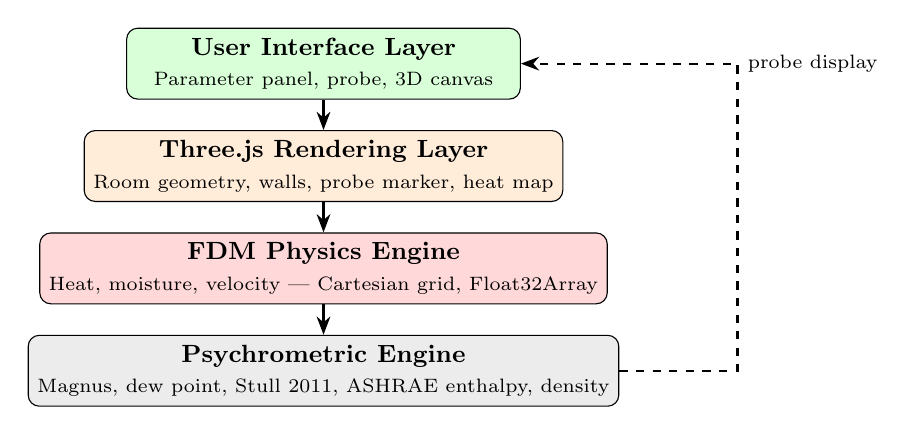
\begin{tikzpicture}[
  box/.style={draw, rounded corners, minimum width=5cm, minimum height=0.9cm,
              align=center, font=\small\bfseries, fill=blue!10},
  arrow/.style={-Stealth, thick}
]
  \node[box, fill=green!15] (ui)     at (0, 3.4) {User Interface Layer\\{\normalfont\scriptsize Parameter panel, probe, 3D canvas}};
  \node[box, fill=orange!15] (render) at (0, 2.1) {Three.js Rendering Layer\\{\normalfont\scriptsize Room geometry, walls, probe marker, heat map}};
  \node[box, fill=red!15] (fdm)     at (0, 0.8) {FDM Physics Engine\\{\normalfont\scriptsize Heat, moisture, velocity --- Cartesian grid, Float32Array}};
  \node[box, fill=gray!15] (psych)  at (0,-0.5) {Psychrometric Engine\\{\normalfont\scriptsize Magnus, dew point, Stull 2011, ASHRAE enthalpy, density}};
  \draw[arrow] (ui)     -- (render);
  \draw[arrow] (render) -- (fdm);
  \draw[arrow] (fdm)    -- (psych);
  \draw[arrow, dashed] (psych.east) -- ++(1.5,0) |- (ui.east) node[midway, right, font=\scriptsize] {probe display};
\end{tikzpicture}
\caption{Application architecture: four coupled layers from physics to UI.}
\label{fig:arch}
\end{figure}

\section{Computational Grid and Indexing}
\label{sec:grid}

The room occupies a user-configurable domain $W\times H\times D$ (default $6\,\text{m}\times3.2\,\text{m}\times5\,\text{m}$). Cell dimensions are given by

\begin{equation}
  \Delta x = \frac{W}{N_x}, \quad \Delta y = \frac{H}{N_y}, \quad \Delta z = \frac{D}{N_z}
  \label{eq:celldims}
\end{equation}

Each cell stores five \texttt{Float32} values, namely $T$, $\omega$, $u$, $v$, $w$. The flat array index is

\begin{equation}
  \text{idx}(i,j,k) = i\,N_y\,N_z + j\,N_z + k
  \label{eq:idx}
\end{equation}

A Boolean mask represents solid obstacles, and the FDM update skips masked cells.

\section{Boundary Conditions}
\label{sec:bc}

\subsection{Wall Conduction}

\begin{equation}
  S_T^\text{wall} = \frac{k_W\,(T_\text{ext} - T)}{\Delta x\,\rho_a\,c_p}
  \label{eq:wall_cond}
\end{equation}

where $k_W$ [W/(m$^2$·K)] is the wall U-value and $c_p=1006$\,J/(kg·K).

\subsection{AC Supply Injection}

Supply cells at the top of the rear wall are overwritten each sub-step according to

\begin{equation}
  T_\text{supply} = T_\text{AC}, \quad \omega_\text{supply} = \min\!\left(\omega_\text{RH}(T_\text{AC}-10, 90\%), \; \omega_\text{init} \times 1.2\right)
  \label{eq:ac}
\end{equation}

\subsection{Door Air Exchange}

\begin{equation}
  F_\text{exch} = 0.4\left(1 + \min\!\left(5,\, \frac{|\rho_\text{ext} - \rho_\text{cell}|}{1.2} \times 15\right)
  + \min\!\left(5,\, \frac{|P_\text{ext} - P_\text{cell}|}{80}\right)\right)
  \label{eq:door}
\end{equation}

The expression captures buoyancy-driven (stack effect, $\propto\Delta\rho$) and pressure-driven ($\propto\Delta P$) exchange.

\section{Heat-Map Colour Mapping}
\label{sec:heatmap}

The Three.js heat-map mode maps temperature to a blue-to-red hue:

\begin{equation}
  H = \frac{(1 - f) \times 240}{360}, \quad f = \text{clamp}\!\left(\frac{T - T_\text{min}}{T_\text{max} - T_\text{min}}, 0, 1\right)
  \label{eq:heatmap}
\end{equation}

\section{Simulation Loop}
\label{sec:simloop}

\begin{figure}[H]
\centering
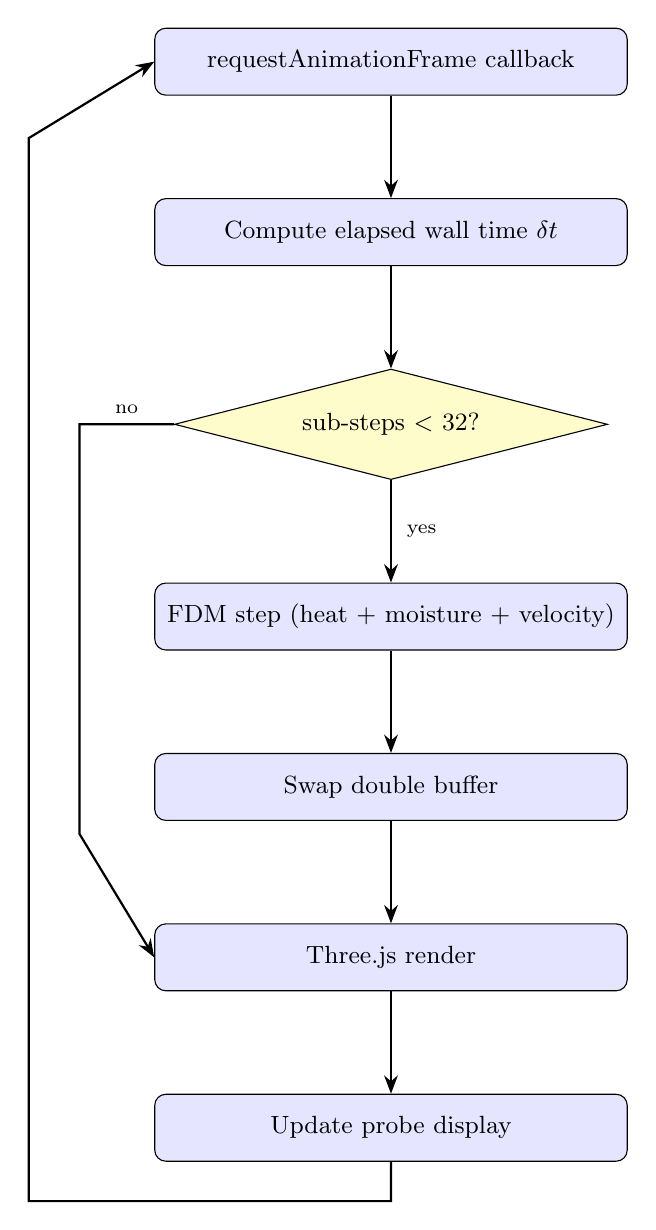
\begin{tikzpicture}[
  proc/.style={draw, rounded corners, minimum width=6cm, minimum height=0.85cm,
               align=center, font=\small, fill=blue!10},
  dec/.style={draw, diamond, aspect=2.8, minimum width=5.5cm,
              align=center, font=\small, fill=yellow!20},
  arrow/.style={-Stealth, thick},
  node distance=1.3cm
]
  \node[proc]                  (raf)    {requestAnimationFrame callback};
  \node[proc, below=of raf]    (dt)     {Compute elapsed wall time $\delta t$};
  \node[dec,  below=of dt]     (cfl)    {sub-steps $<$ 32?};
  \node[proc, below=of cfl]    (fdm)    {FDM step (heat + moisture + velocity)};
  \node[proc, below=of fdm]    (swap)   {Swap double buffer};
  \node[proc, below=of swap]   (render) {Three.js render};
  \node[proc, below=of render] (probe)  {Update probe display};

  \draw[arrow] (raf)    -- (dt);
  \draw[arrow] (dt)     -- (cfl);
  \draw[arrow] (cfl)    -- node[right=2pt, font=\scriptsize]{yes} (fdm);
  \draw[arrow] (fdm)    -- (swap);
  \draw[arrow] (swap)   -- (render);
  \draw[arrow] (render) -- (probe);

  \draw[arrow] (cfl.west) -- ++(-1.2,0)
      node[midway, above, font=\scriptsize]{no}
      -- ++(0,-5.2)
      -- (render.west);

  \draw[arrow] (probe.south) -- ++(0,-0.5)
      -- ++(-4.6,0)
      -- ++(0,13.5)
      -- (raf.west);
\end{tikzpicture}
\caption{Simulation loop: up to 32 FDM sub-steps per animation frame.}
\label{fig:simloop}
\end{figure}

\section{Heat Source Models}
\label{sec:sources}

\begin{table}[H]
\centering
\caption{Internal heat and moisture source terms.}
\label{tab:sources}
\renewcommand{\arraystretch}{1.2}
\begin{tabular}{lllc}
\toprule
\textbf{Source} & \textbf{Heat [W/cell]} & \textbf{Moisture [g/kg$_{da}$/s]} & \textbf{Location}\\
\midrule
Human metabolic & 80\,W/person    & $1.1\times10^{-2}$ & Floor cells\\
Desktop PC       & 120\,W          & ---                & Desk cells\\
Laptop PC        & 50\,W           & ---                & Desk cells\\
LED lights       & 10\,W/fixture   & ---                & Ceiling cells\\
Solar gain       & User-defined    & ---                & Sunroof cells\\
Infiltration     & ---             & $(ACH/3600)\!\times\!0.1\!\times\!\Delta\omega$ & Boundary cells\\
\bottomrule
\end{tabular}
\end{table}










%==================================================================
\chapter{Results and Discussion}
\label{ch:results}
%==================================================================

\section{Baseline Case}
\label{sec:baseline}

The baseline room measures $6\,\text{m}\times3.2\,\text{m}\times5\,\text{m}$ and starts at $T=28$°C and RH\,=\,60\%, with AC setpoint 22°C, two occupants, two desktop PCs, four LED fixtures, a closed door, and external $T=35$°C. Results are for quasi-steady state after $\approx300$ simulated seconds.

\subsection{Thermal Stratification}

Figure~\ref{fig:stratification} shows the vertical temperature profile at the room centreline. The vertical gradient is $\approx1.2$°C/m, consistent with ASHRAE~55-2020 comfort guidelines \cite{ashrae55}.

\begin{figure}[H]
\centering
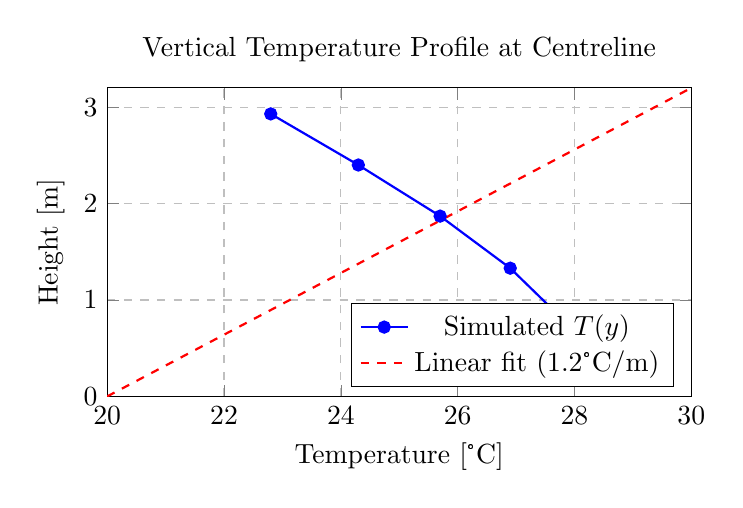
\begin{tikzpicture}
\begin{axis}[
  width=9cm, height=5.5cm,
  xlabel={Temperature [°C]},
  ylabel={Height [m]},
  xmin=20, xmax=30, ymin=0, ymax=3.2,
  grid=major, grid style={dashed, gray!50},
  legend pos=south east,
  title={Vertical Temperature Profile at Centreline}
]
\addplot[blue, thick, mark=*] coordinates {
  (28.4, 0.27) (27.8, 0.80) (26.9, 1.33) (25.7, 1.87) (24.3, 2.40) (22.8, 2.93)
};
\addlegendentry{Simulated $T(y)$}
\addplot[red, dashed, thick] coordinates {(20,0) (30,3.2)};
\addlegendentry{Linear fit ($1.2$°C/m)}
\end{axis}
\end{tikzpicture}
\caption{Vertical temperature profile at centreline ($x=3$\,m, $z=2.5$\,m), quasi-steady state.}
\label{fig:stratification}
\end{figure}

\subsection{Psychrometric State at Representative Locations}

\begin{table}[H]
\centering
\caption{Psychrometric state at representative probe locations (quasi-steady).}
\label{tab:psychro}
\renewcommand{\arraystretch}{1.2}
\begin{tabular}{lcccccc}
\toprule
\textbf{Location} & $T$ [°C] & $\omega$ [g/kg] & RH [\%] & $T_{dp}$ [°C] & $T_{wb}$ [°C] & $h$ [kJ/kg]\\
\midrule
Floor centre    & 28.4 & 11.8 & 55.2 & 18.9 & 22.1 & 58.6\\
Desk (PC zone)  & 29.1 & 12.2 & 54.0 & 19.1 & 22.4 & 60.3\\
Mid height      & 25.7 & 10.5 & 51.8 & 15.4 & 19.8 & 52.5\\
AC supply zone  & 22.8 &  8.7 & 47.5 & 11.5 & 17.3 & 45.1\\
\bottomrule
\end{tabular}
\end{table}

Humidity reaches quasi-steady state at $\approx55\%$ RH near occupants and $\approx48\%$ near the AC supply. When the door is opened, the density-driven exchange term (equation~\ref{eq:door}) raises zone-average temperature by $\approx1.4$°C and RH by $\approx3\%$ over 60 simulated seconds. The Boussinesq term (equation~\ref{eq:momentum}) drives a counter-rotating convection cell with peak vertical velocity $v_\text{max}\approx0.15$\,m/s, below the ISO~7730 comfort limit of 0.2\,m/s \cite{iso7730}.









%==================================================================
\chapter{Conclusion and Future Work}
\label{ch:conclusion}
%==================================================================

\section{Summary}
\label{sec:summary}

A physically self-consistent, real-time 3D thermal simulation of a conditioned room is achievable within a browser-based application on commodity hardware. The implementation couples heat, moisture, and momentum transport in a 3D FDM engine on a Cartesian grid with explicit Forward Euler time-stepping and CFL-limited sub-stepping; it evaluates a complete ASHRAE psychrometric engine (equations~\ref{eq:magnus} to \ref{eq:density}) for every grid cell at every time step; it models AC injection, wall conduction, solar gain, occupant and equipment loads, infiltration, and density-driven door exchange; it renders a Three.js 3D interactive scene with dynamic wall opacity, a psychrometric probe, and a blue-to-red heat-map; and it provides an Electron.js desktop packaging workflow.

\section{Limitations}

The coarse Cartesian grid cannot resolve boundary-layer effects or the fine structure of the AC supply jet, and without a pressure projection solver \cite{chorin1968} the velocity field does not strictly satisfy the divergence-free condition. Long-wave radiative exchange between surfaces is not modelled, and the first-order upwind scheme introduces numerical diffusion.

\section{Future Work: PINNs}
\label{sec:future}

The most promising extension is to replace the FDM solver with a Physics-Informed Neural Network (PINN) surrogate \cite{raissi2019}. PINNs embed the governing PDEs (equations~\ref{eq:heat} to \ref{eq:momentum}) directly into the training loss:

\begin{equation}
  \mathcal{L} = \mathcal{L}_\text{data} + \lambda_1\mathcal{L}_\text{PDE} + \lambda_2\mathcal{L}_\text{BC}
  \label{eq:pinn_loss}
\end{equation}

where $\mathcal{L}_\text{data}$ penalises deviation from sensor measurements, $\mathcal{L}_\text{PDE}$ penalises PDE residuals at collocation points, and $\mathcal{L}_\text{BC}$ penalises boundary-condition errors. Once trained, the network evaluates the full 3D thermal field in a single forward pass ($<1$\,ms on a GPU), enabling live sensor fusion and resolution-independent queries. Additional future directions include a pressure projection solver, long-wave radiative exchange, a multi-zone network model, and CO$_2$ concentration tracking.









%==================================================================
% List of Important Symbols
%==================================================================
\chapter*{List of Important Symbols}
\addcontentsline{toc}{chapter}{List of Important Symbols}

\begin{longtable}{p{2.2cm} p{8cm} p{2.8cm}}
\toprule
\textbf{Symbol} & \textbf{Description} & \textbf{Units}\\
\midrule
\endhead
$T$ & Dry-bulb temperature & °C\\
$T_K$ & Absolute temperature & K\\
$T_{dp}$ & Dew-point temperature & °C\\
$T_{wb}$ & Wet-bulb temperature & °C\\
$\omega$ & Humidity ratio & kg$_w$/kg$_{da}$\\
$\phi$ & Relative humidity & \%\\
$p_v$ & Partial pressure of water vapour & Pa\\
$p_{ws}$ & Saturation vapour pressure & Pa\\
$P$ & Atmospheric pressure & Pa\\
$h$ & Specific enthalpy of moist air & kJ/kg$_{da}$\\
$\rho$ & Moist-air density & kg/m$^3$\\
$\alpha$ & Thermal diffusivity of air & m$^2$/s\\
$D_m$ & Mass diffusivity of water vapour & m$^2$/s\\
$\nu$ & Kinematic viscosity of air & m$^2$/s\\
$\beta$ & Volumetric thermal expansion coefficient & K$^{-1}$\\
$c_p$ & Specific heat of dry air & J/(kg·K)\\
$R_{da}$, $R_v$ & Gas constants of dry air / water vapour & J/(kg·K)\\
$k_W$ & Wall U-value & W/(m$^2$·K)\\
$\Delta t$ & Time step & s\\
$\Delta x,\Delta y,\Delta z$ & Cell dimensions & m\\
$\mathbf{v}=(u,v,w)$ & Velocity vector & m/s\\
$S_T$, $S_\omega$ & Volumetric heat / moisture source & °C/s, kg$_w$/(kg$_{da}$·s)\\
ACH & Air changes per hour & h$^{-1}$\\
FDM, CFL, PINN & Finite Difference Method / Courant--Friedrichs--Lewy / Physics-Informed Neural Network & --\\
\bottomrule
\end{longtable}










%==================================================================
% References
%==================================================================
\renewcommand{\bibname}{References}
\begin{thebibliography}{99}
\addcontentsline{toc}{chapter}{References}

\bibitem{iea2022}
International Energy Agency, ``Buildings,'' IEA Technology Report, Paris, 2022.

\bibitem{ashrae2021}
ASHRAE Handbook: Fundamentals (SI), ASHRAE, Atlanta, GA, 2021.

\bibitem{crawley2001}
D.\ B.\ Crawley \emph{et al.}, ``EnergyPlus: Creating a new-generation building energy simulation program,'' \textit{Energy and Buildings}, vol.\ 33, no.\ 4, 2001.

\bibitem{grieves2014}
M.\ Grieves and J.\ Vickers, ``Digital twin: Mitigating unpredictable emergent behavior in complex systems,'' in \textit{Transdisciplinary Perspectives on Complex Systems}, Springer, 2017.

\bibitem{august1828}
F.\ W.\ August, ``\"{U}ber die Verdunstungsk\"{a}lte,'' \textit{Annalen der Physik und Chemie}, vol.\ 5, 1828.

\bibitem{alduchov1996}
O.\ A.\ Alduchov and R.\ E.\ Eskridge, ``Improved Magnus form approximation of saturation vapor pressure,'' \textit{J.\ Appl.\ Meteorology}, vol.\ 35, no.\ 4, 1996.

\bibitem{stull2011}
R.\ Stull, ``Wet-bulb temperature from relative humidity and air temperature,'' \textit{J.\ Appl.\ Meteorology Climatology}, vol.\ 50, no.\ 11, 2011.

\bibitem{boussinesq1903}
J.\ Boussinesq, \textit{Th\'{e}orie analytique de la chaleur}, vol.\ 2. Paris: Gauthier-Villars, 1903.

\bibitem{courant1928}
R.\ Courant, K.\ Friedrichs, and H.\ Lewy, ``\"{U}ber die partiellen Differenzengleichungen,'' \textit{Math.\ Annalen}, vol.\ 100, 1928.

\bibitem{winkelmann1993}
F.\ C.\ Winkelmann \emph{et al.}, ``DOE-2 Supplement: Version 2.1E,'' LBNL Tech.\ Rep.\ LBL-34947, 1993.

\bibitem{pod2002}
L.\ Sirovich, ``Turbulence and the dynamics of coherent structures,'' \textit{Q.\ Appl.\ Math.}, vol.\ 45, no.\ 3, 1987.

\bibitem{zhao2020}
L.\ Zhao, Y.\ Zhang, and F.\ Duarte, ``A digital twin framework for real-time monitoring of building thermal systems,'' \textit{Automation in Construction}, vol.\ 118, 2020.

\bibitem{deng2022}
Z.\ Deng, Q.\ Chen, and L.\ Liu, ``Predictive control of building HVAC using PINN co-simulation,'' \textit{Building and Environment}, vol.\ 207, 2022.

\bibitem{electron}
Electron.js Contributors, ``Electron: Build cross-platform desktop apps,'' GitHub, 2024.

\bibitem{ashrae55}
ANSI/ASHRAE Standard 55-2020, \textit{Thermal Environmental Conditions for Human Occupancy}. ASHRAE, 2020.

\bibitem{iso7730}
ISO 7730:2005, \textit{Ergonomics of the thermal environment}. Geneva: ISO, 2005.

\bibitem{raissi2019}
M.\ Raissi, P.\ Perdikaris, and G.\ E.\ Karniadakis, ``Physics-informed neural networks,'' \textit{J.\ Computational Physics}, vol.\ 378, 2019.

\bibitem{chorin1968}
A.\ J.\ Chorin, ``Numerical solution of the Navier-Stokes equations,'' \textit{Math.\ Computation}, vol.\ 22, no.\ 104, 1968.

\end{thebibliography}

\end{document}